\documentclass[11pt,a4paper]{book}
\usepackage[utf8]{inputenc}
\usepackage{amsmath}
\usepackage{amsfonts}
\usepackage{amssymb}
\usepackage{graphicx}
\usepackage{url}
\usepackage{lipsum}
\usepackage{marginnote}
\usepackage{todonotes}

\author{FrontEndART Szoftver Kft.}
\title{Developer's Guide of the CROSSMINER Advanced Integrated Development Environments Plug-in}
\date{Version 1.0.0.rev0}

\makeatletter
\renewcommand{\maketitle}{
\vspace*{.1\textheight}
\begin{center}
	
\includegraphics[width=.6\textwidth]{pic/CROSSMINER-logo-large.png}
\end{center}
\begin{center}
	\Huge\@title
\end{center}
\vfill
\begin{center}
	\large\@author\\\@date{} $\bullet$ \today
\end{center}
}
\makeatother

\newcommand{\placeholder}[1]{$\left\langle\text{#1}\right\rangle$}

\newcommand{\SHALL}{\colorbox{red!25}{\textsc{shall}}}
\newcommand{\SHOULD}{\colorbox{orange!25}{\textsc{should}}}
\newcommand{\MAY}{\colorbox{cyan!25}{\textsc{may}}}

\newcommand{\status}[1]{\textbf{Status:} #1}
\newcommand{\todom}{\textcolor{gray}{to do}}
\newcommand{\waitingForServer}{\textcolor{red}{waiting for server side implementation}}
\newcommand{\inprogress}{\textcolor{orange}{partially done}}
\newcommand{\done}{\textcolor{green}{done}}

\newcommand{\unknown}{\colorbox{yellow}{???}}

\newcommand{\req}[4][\todom]{\medskip\marginnote{
\includegraphics[width=2.75em]{pic/contract}}\noindent\textbf{\textsf{Requirement #2}} #4  \status{#1}\\\noindent\textit{#3}\bigskip\par}

\begin{document}
	
\begin{titlepage}
	\maketitle
\end{titlepage}

\chapter{Development Processes}

The general layout of the development and testing process are shown on Figure~\ref{fig:version}

\begin{figure}[h]
	\centering
	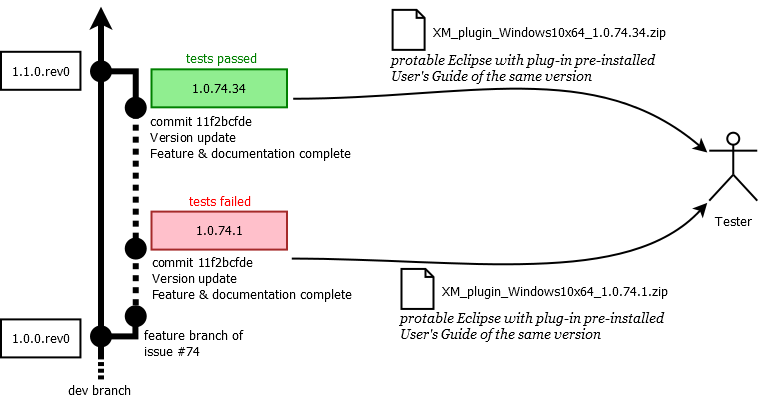
\includegraphics[width=\linewidth]{pic/version.png}
	\caption{Overview of the testing and development process}
	\label{fig:version}
\end{figure}


\section{Versions}
The version number consists of three parts separated by period. It follows the layout \emph{\placeholder{main}.\placeholder{sub}.\placeholder{issue}.rev\placeholder{revision}}. To understand when and how to change these parts please consider the following guide.

\begin{description}
	\item[Increasing main version] Request rights of lead developer or above. It will be increased when the current version are shipped and demonstrated to the (whole) consortium.
	\item[Increasing sub version] Could be changed by any participant. Increase it by one respecting to the current version of the \texttt{dev} branch when a new feature are finished, passed all required tests and merged into the current development version (on \texttt{dev} branch). Reset it to 0 every time main version number increases. 
	\item[Changing issue number] You have to set this part to be equal the identification number of the current issue associated to the feature branch you are on. Set it 0 on non-feature branches.
	\item[Incrementing the revision] Could be changed by any participant. Increment it by one, before you send a new version for testing. It could be the first version containing a testable new feature or any fixes applied due to testers concerns. Reset it to 0 at the beginning of each new feature branch.
\end{description}

There are some additional rules need to consider, partially implicated by the these statements. You have to follow these as well the previous ones.

\begin{description}
	\item[Development versions] Each version on the \texttt{dev} branch should follow this scheme: \emph{\placeholder{main}.\placeholder{sub}.0.rev0}, for example \emph{1.12.0.rev0}.
	\item[Testable versions] Each version sent for testing should follow this scheme: \emph{\placeholder{main}.\placeholder{sub}.\placeholder{current-issue}.rev\placeholder{revision}}, for example \emph{2.23.42.rev11}.
	\item[Version tagging] Each version should be explicitly tagged in the Git repository using the following commands (if your HEAD points to the relevant commit):\\\texttt{git tag \placeholder{version}\\git push origin \placeholder{version}}
	\item[Issue-branch-feature tracibility] Each feature branch has to have a single and unique issue. Do not change (create new) version off the plug-in after merging a branch contains only refactoring without any new features or fixes.
	\item[Tracability of User's Guide] The User's Guide (this document) has to follow the version any version changes. You have to update the guide before you change the version number.
\end{description}

\section{Structure of Releases}

After chancing the version you have to assemble a new release package. By doing so please follow these rules.

\begin{description}
	\item[Naming] Each release package should be named by the following scheme: \emph{XM\_plugin\_\placeholder{operation-system}\_v\placeholder{version}.zip},\\for example \texttt{XM\_plugin\_Windows10x64\_2.23.0.rev0}
	\item[Content] Each release should consist of a single, self-contained compressed folder, containing a portable Eclipse with the plug-in pre-installed.\footnote{Except in the cases, when the goal of testing is installation.}
	\item[Placing Documentation] The relevant version of this document should be placed in the root folder of the compressed package in PDF format.
\end{description}

\section{Testing}

Each feature and function should be tested against expected functionality described in this document. Any discrepancies should be reported.

\begin{description}
	\item[Reporting failed tests] All failed test should be reported using a dedicated issue recorded in the project. \url{https://git.sed.hu/geryxyz/crossminer/issues/new}
	\item[Content of the report] Each report should contain a detailed description of the action and condition of test to be repeatable. You have to specify the concrete version in which the divergence occur and the exact place in this document where the feature was described.
	\item[Goal of testing] As a tester you have to ensure that each features are working as described in this document with reasonable reliability.
\end{description}


\end{document}